\chapter{Metodologia}
% [AGENT: INSERIR TEXTO DA METODOLOGIA AQUI]
% Dica: Descreva o tipo de pesquisa, os instrumentos de coleta de dados e os métodos de análise.

Apresentação da metodologia do trabalho e procedimentos adotados na pesquisa. Como representação visual dos módulos do sistema, a \autoref{fig:metodologia-exemplo} descreve a arquitetura proposta.

\begin{figure}[!htbp]
    \centering
    \caption{Visão Geral da Metodologia e Arquitetura Proposta}
    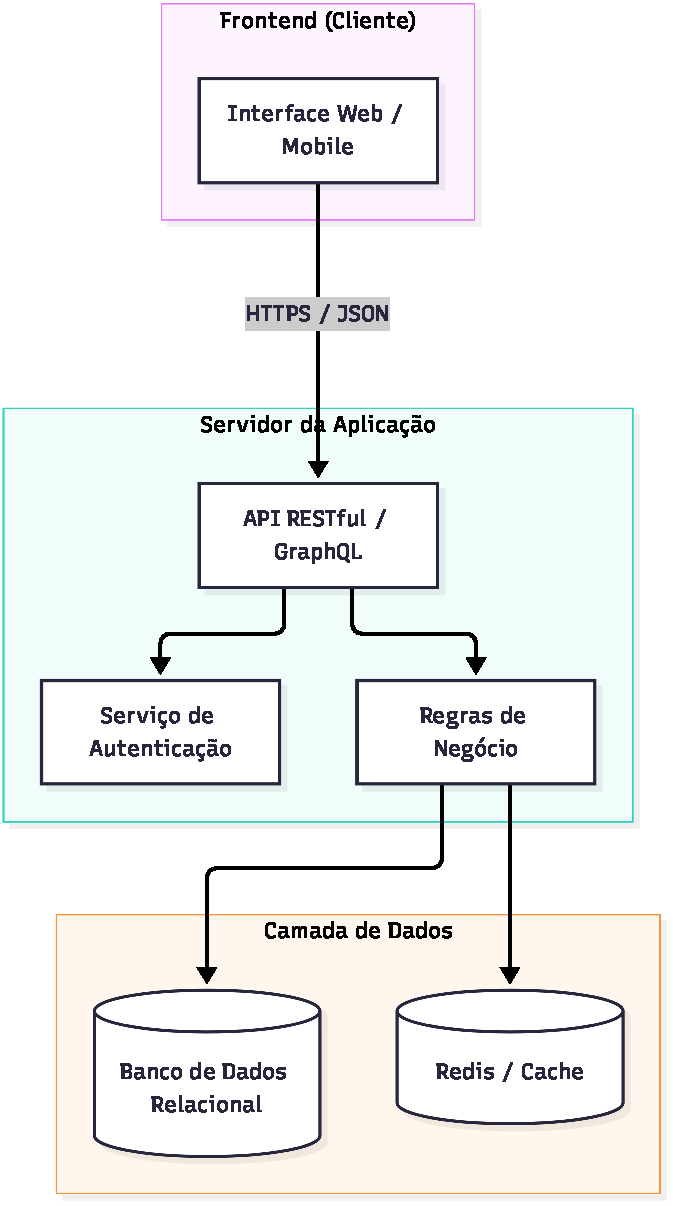
\includegraphics[width=0.85\textwidth,height=0.45\textheight,keepaspectratio]{figuras/exemplo-diagrama.pdf}
    \fonte{Elaborado pelo autor (\the\year).}
    \label{fig:metodologia-exemplo}
\end{figure}

\section{Exemplo de Listagem de Código-Fonte}

Para trechos de algoritmos, consultas ou contratos de integração, utiliza-se o ambiente \texttt{lstlisting} já estilizado no preâmbulo institucional, como ilustrado no Código~\ref{lst:exemplo-consulta}.

\begin{lstlisting}[language=Python, caption={Exemplo de função de validação estruturada em Python}, label={lst:exemplo-consulta}]
def validar_registro(registro: dict) -> bool:
    campos_obrigatorios = ("matricula", "modalidade", "status")
    return all(campo in registro and registro[campo] for campo in campos_obrigatorios)
\end{lstlisting}
